\documentclass{report}

%%%%%%%%%%%%%%%%%%%%%%%%%%%%%%%%%
% PACKAGE IMPORTS
%%%%%%%%%%%%%%%%%%%%%%%%%%%%%%%%%


\usepackage[tmargin=2cm,rmargin=1in,lmargin=1in,margin=0.85in,bmargin=2cm,footskip=.2in]{geometry}
\usepackage{amsmath,amsfonts,amsthm,amssymb,mathtools}
\usepackage[varbb]{newpxmath}
\usepackage{xfrac}
\usepackage[makeroom]{cancel}
\usepackage{mathtools}
\usepackage{bookmark}
\usepackage{enumitem}
\usepackage{hyperref,theoremref}
\hypersetup{
	pdftitle={Assignment},
	colorlinks=true, linkcolor=doc!90,
	bookmarksnumbered=true,
	bookmarksopen=true
}
\usepackage[most,many,breakable]{tcolorbox}
\usepackage{xcolor}
\usepackage{varwidth}
\usepackage{varwidth}
\usepackage{etoolbox}
%\usepackage{authblk}
\usepackage{nameref}
\usepackage{multicol,array}
\usepackage{tikz-cd}
\usepackage[ruled,vlined,linesnumbered]{algorithm2e}
\usepackage{comment} % enables the use of multi-line comments (\ifx \fi) 
\usepackage{import}
\usepackage{xifthen}
\usepackage{pdfpages}
\usepackage{transparent}

\newcommand\mycommfont[1]{\footnotesize\ttfamily\textcolor{blue}{#1}}
\SetCommentSty{mycommfont}
\newcommand{\incfig}[1]{%
    \def\svgwidth{\columnwidth}
    \import{./figures/}{#1.pdf_tex}
}

\usepackage{tikzsymbols}
\usepackage{tikz}
\usepackage[siunitx]{circuitikz}
\renewcommand\qedsymbol{$\Laughey$}


%\usepackage{import}
%\usepackage{xifthen}
%\usepackage{pdfpages}
%\usepackage{transparent}


%%%%%%%%%%%%%%%%%%%%%%%%%%%%%%
% SELF MADE COLORS
%%%%%%%%%%%%%%%%%%%%%%%%%%%%%%



\definecolor{myg}{RGB}{56, 140, 70}
\definecolor{myb}{RGB}{45, 111, 177}
\definecolor{myr}{RGB}{199, 68, 64}
\definecolor{mytheorembg}{HTML}{F2F2F9}
\definecolor{mytheoremfr}{HTML}{00007B}
\definecolor{mylenmabg}{HTML}{FFFAF8}
\definecolor{mylenmafr}{HTML}{983b0f}
\definecolor{mypropbg}{HTML}{f2fbfc}
\definecolor{mypropfr}{HTML}{191971}
\definecolor{myexamplebg}{HTML}{F2FBF8}
\definecolor{myexamplefr}{HTML}{88D6D1}
\definecolor{myexampleti}{HTML}{2A7F7F}
\definecolor{mydefinitbg}{HTML}{E5E5FF}
\definecolor{mydefinitfr}{HTML}{3F3FA3}
\definecolor{notesgreen}{RGB}{0,162,0}
\definecolor{myp}{RGB}{197, 92, 212}
\definecolor{mygr}{HTML}{2C3338}
\definecolor{myred}{RGB}{127,0,0}
\definecolor{myyellow}{RGB}{169,121,69}
\definecolor{myexercisebg}{HTML}{F2FBF8}
\definecolor{myexercisefg}{HTML}{88D6D1}


%%%%%%%%%%%%%%%%%%%%%%%%%%%%
% TCOLORBOX SETUPS
%%%%%%%%%%%%%%%%%%%%%%%%%%%%

\setlength{\parindent}{1cm}
%================================
% THEOREM BOX
%================================

\tcbuselibrary{theorems,skins,hooks}
\newtcbtheorem[number within=section]{Theorem}{Theorem}
{%
	enhanced,
	breakable,
	colback = mytheorembg,
	frame hidden,
	boxrule = 0sp,
	borderline west = {2pt}{0pt}{mytheoremfr},
	sharp corners,
	detach title,
	before upper = \tcbtitle\par\smallskip,
	coltitle = mytheoremfr,
	fonttitle = \bfseries\sffamily,
	description font = \mdseries,
	separator sign none,
	segmentation style={solid, mytheoremfr},
}
{th}

\tcbuselibrary{theorems,skins,hooks}
\newtcbtheorem[number within=chapter]{theorem}{Theorem}
{%
	enhanced,
	breakable,
	colback = mytheorembg,
	frame hidden,
	boxrule = 0sp,
	borderline west = {2pt}{0pt}{mytheoremfr},
	sharp corners,
	detach title,
	before upper = \tcbtitle\par\smallskip,
	coltitle = mytheoremfr,
	fonttitle = \bfseries\sffamily,
	description font = \mdseries,
	separator sign none,
	segmentation style={solid, mytheoremfr},
}
{th}


\tcbuselibrary{theorems,skins,hooks}
\newtcolorbox{Theoremcon}
{%
	enhanced
	,breakable
	,colback = mytheorembg
	,frame hidden
	,boxrule = 0sp
	,borderline west = {2pt}{0pt}{mytheoremfr}
	,sharp corners
	,description font = \mdseries
	,separator sign none
}

%================================
% Corollery
%================================
\tcbuselibrary{theorems,skins,hooks}
\newtcbtheorem[number within=section]{Corollary}{Corollary}
{%
	enhanced
	,breakable
	,colback = myp!10
	,frame hidden
	,boxrule = 0sp
	,borderline west = {2pt}{0pt}{myp!85!black}
	,sharp corners
	,detach title
	,before upper = \tcbtitle\par\smallskip
	,coltitle = myp!85!black
	,fonttitle = \bfseries\sffamily
	,description font = \mdseries
	,separator sign none
	,segmentation style={solid, myp!85!black}
}
{th}
\tcbuselibrary{theorems,skins,hooks}
\newtcbtheorem[number within=chapter]{corollary}{Corollary}
{%
	enhanced
	,breakable
	,colback = myp!10
	,frame hidden
	,boxrule = 0sp
	,borderline west = {2pt}{0pt}{myp!85!black}
	,sharp corners
	,detach title
	,before upper = \tcbtitle\par\smallskip
	,coltitle = myp!85!black
	,fonttitle = \bfseries\sffamily
	,description font = \mdseries
	,separator sign none
	,segmentation style={solid, myp!85!black}
}
{th}


%================================
% LENMA
%================================

\tcbuselibrary{theorems,skins,hooks}
\newtcbtheorem[number within=section]{Lenma}{Lenma}
{%
	enhanced,
	breakable,
	colback = mylenmabg,
	frame hidden,
	boxrule = 0sp,
	borderline west = {2pt}{0pt}{mylenmafr},
	sharp corners,
	detach title,
	before upper = \tcbtitle\par\smallskip,
	coltitle = mylenmafr,
	fonttitle = \bfseries\sffamily,
	description font = \mdseries,
	separator sign none,
	segmentation style={solid, mylenmafr},
}
{th}

\tcbuselibrary{theorems,skins,hooks}
\newtcbtheorem[number within=chapter]{lenma}{Lenma}
{%
	enhanced,
	breakable,
	colback = mylenmabg,
	frame hidden,
	boxrule = 0sp,
	borderline west = {2pt}{0pt}{mylenmafr},
	sharp corners,
	detach title,
	before upper = \tcbtitle\par\smallskip,
	coltitle = mylenmafr,
	fonttitle = \bfseries\sffamily,
	description font = \mdseries,
	separator sign none,
	segmentation style={solid, mylenmafr},
}
{th}


%================================
% PROPOSITION
%================================

\tcbuselibrary{theorems,skins,hooks}
\newtcbtheorem[number within=section]{Prop}{Proposition}
{%
	enhanced,
	breakable,
	colback = mypropbg,
	frame hidden,
	boxrule = 0sp,
	borderline west = {2pt}{0pt}{mypropfr},
	sharp corners,
	detach title,
	before upper = \tcbtitle\par\smallskip,
	coltitle = mypropfr,
	fonttitle = \bfseries\sffamily,
	description font = \mdseries,
	separator sign none,
	segmentation style={solid, mypropfr},
}
{th}

\tcbuselibrary{theorems,skins,hooks}
\newtcbtheorem[number within=chapter]{prop}{Proposition}
{%
	enhanced,
	breakable,
	colback = mypropbg,
	frame hidden,
	boxrule = 0sp,
	borderline west = {2pt}{0pt}{mypropfr},
	sharp corners,
	detach title,
	before upper = \tcbtitle\par\smallskip,
	coltitle = mypropfr,
	fonttitle = \bfseries\sffamily,
	description font = \mdseries,
	separator sign none,
	segmentation style={solid, mypropfr},
}
{th}


%================================
% CLAIM
%================================

\tcbuselibrary{theorems,skins,hooks}
\newtcbtheorem[number within=section]{claim}{Claim}
{%
	enhanced
	,breakable
	,colback = myg!10
	,frame hidden
	,boxrule = 0sp
	,borderline west = {2pt}{0pt}{myg}
	,sharp corners
	,detach title
	,before upper = \tcbtitle\par\smallskip
	,coltitle = myg!85!black
	,fonttitle = \bfseries\sffamily
	,description font = \mdseries
	,separator sign none
	,segmentation style={solid, myg!85!black}
}
{th}



%================================
% Exercise
%================================

\tcbuselibrary{theorems,skins,hooks}
\newtcbtheorem[number within=section]{Exercise}{Exercise}
{%
	enhanced,
	breakable,
	colback = myexercisebg,
	frame hidden,
	boxrule = 0sp,
	borderline west = {2pt}{0pt}{myexercisefg},
	sharp corners,
	detach title,
	before upper = \tcbtitle\par\smallskip,
	coltitle = myexercisefg,
	fonttitle = \bfseries\sffamily,
	description font = \mdseries,
	separator sign none,
	segmentation style={solid, myexercisefg},
}
{th}

\tcbuselibrary{theorems,skins,hooks}
\newtcbtheorem[number within=chapter]{exercise}{Exercise}
{%
	enhanced,
	breakable,
	colback = myexercisebg,
	frame hidden,
	boxrule = 0sp,
	borderline west = {2pt}{0pt}{myexercisefg},
	sharp corners,
	detach title,
	before upper = \tcbtitle\par\smallskip,
	coltitle = myexercisefg,
	fonttitle = \bfseries\sffamily,
	description font = \mdseries,
	separator sign none,
	segmentation style={solid, myexercisefg},
}
{th}

%================================
% EXAMPLE BOX
%================================

\newtcbtheorem[number within=section]{Example}{Example}
{%
	colback = myexamplebg
	,breakable
	,colframe = myexamplefr
	,coltitle = myexampleti
	,boxrule = 1pt
	,sharp corners
	,detach title
	,before upper=\tcbtitle\par\smallskip
	,fonttitle = \bfseries
	,description font = \mdseries
	,separator sign none
	,description delimiters parenthesis
}
{ex}

\newtcbtheorem[number within=chapter]{example}{Example}
{%
	colback = myexamplebg
	,breakable
	,colframe = myexamplefr
	,coltitle = myexampleti
	,boxrule = 1pt
	,sharp corners
	,detach title
	,before upper=\tcbtitle\par\smallskip
	,fonttitle = \bfseries
	,description font = \mdseries
	,separator sign none
	,description delimiters parenthesis
}
{ex}

%================================
% DEFINITION BOX
%================================

\newtcbtheorem[number within=section]{Definition}{Definition}{enhanced,
	before skip=2mm,after skip=2mm, colback=red!5,colframe=red!80!black,boxrule=0.5mm,
	attach boxed title to top left={xshift=1cm,yshift*=1mm-\tcboxedtitleheight}, varwidth boxed title*=-3cm,
	boxed title style={frame code={
					\path[fill=tcbcolback]
					([yshift=-1mm,xshift=-1mm]frame.north west)
					arc[start angle=0,end angle=180,radius=1mm]
					([yshift=-1mm,xshift=1mm]frame.north east)
					arc[start angle=180,end angle=0,radius=1mm];
					\path[left color=tcbcolback!60!black,right color=tcbcolback!60!black,
						middle color=tcbcolback!80!black]
					([xshift=-2mm]frame.north west) -- ([xshift=2mm]frame.north east)
					[rounded corners=1mm]-- ([xshift=1mm,yshift=-1mm]frame.north east)
					-- (frame.south east) -- (frame.south west)
					-- ([xshift=-1mm,yshift=-1mm]frame.north west)
					[sharp corners]-- cycle;
				},interior engine=empty,
		},
	fonttitle=\bfseries,
	title={#2},#1}{def}
\newtcbtheorem[number within=chapter]{definition}{Definition}{enhanced,
	before skip=2mm,after skip=2mm, colback=red!5,colframe=red!80!black,boxrule=0.5mm,
	attach boxed title to top left={xshift=1cm,yshift*=1mm-\tcboxedtitleheight}, varwidth boxed title*=-3cm,
	boxed title style={frame code={
					\path[fill=tcbcolback]
					([yshift=-1mm,xshift=-1mm]frame.north west)
					arc[start angle=0,end angle=180,radius=1mm]
					([yshift=-1mm,xshift=1mm]frame.north east)
					arc[start angle=180,end angle=0,radius=1mm];
					\path[left color=tcbcolback!60!black,right color=tcbcolback!60!black,
						middle color=tcbcolback!80!black]
					([xshift=-2mm]frame.north west) -- ([xshift=2mm]frame.north east)
					[rounded corners=1mm]-- ([xshift=1mm,yshift=-1mm]frame.north east)
					-- (frame.south east) -- (frame.south west)
					-- ([xshift=-1mm,yshift=-1mm]frame.north west)
					[sharp corners]-- cycle;
				},interior engine=empty,
		},
	fonttitle=\bfseries,
	title={#2},#1}{def}



%================================
% Solution BOX
%================================

\makeatletter
\newtcbtheorem{question}{Question}{enhanced,
	breakable,
	colback=white,
	colframe=myb!80!black,
	attach boxed title to top left={yshift*=-\tcboxedtitleheight},
	fonttitle=\bfseries,
	title={#2},
	boxed title size=title,
	boxed title style={%
			sharp corners,
			rounded corners=northwest,
			colback=tcbcolframe,
			boxrule=0pt,
		},
	underlay boxed title={%
			\path[fill=tcbcolframe] (title.south west)--(title.south east)
			to[out=0, in=180] ([xshift=5mm]title.east)--
			(title.center-|frame.east)
			[rounded corners=\kvtcb@arc] |-
			(frame.north) -| cycle;
		},
	#1
}{def}
\makeatother

%================================
% SOLUTION BOX
%================================

\makeatletter
\newtcolorbox{solution}{enhanced,
	breakable,
	colback=white,
	colframe=myg!80!black,
	attach boxed title to top left={yshift*=-\tcboxedtitleheight},
	title=Solution,
	boxed title size=title,
	boxed title style={%
			sharp corners,
			rounded corners=northwest,
			colback=tcbcolframe,
			boxrule=0pt,
		},
	underlay boxed title={%
			\path[fill=tcbcolframe] (title.south west)--(title.south east)
			to[out=0, in=180] ([xshift=5mm]title.east)--
			(title.center-|frame.east)
			[rounded corners=\kvtcb@arc] |-
			(frame.north) -| cycle;
		},
}
\makeatother

%================================
% Question BOX
%================================

\makeatletter
\newtcbtheorem{qstion}{Question}{enhanced,
	breakable,
	colback=white,
	colframe=mygr,
	attach boxed title to top left={yshift*=-\tcboxedtitleheight},
	fonttitle=\bfseries,
	title={#2},
	boxed title size=title,
	boxed title style={%
			sharp corners,
			rounded corners=northwest,
			colback=tcbcolframe,
			boxrule=0pt,
		},
	underlay boxed title={%
			\path[fill=tcbcolframe] (title.south west)--(title.south east)
			to[out=0, in=180] ([xshift=5mm]title.east)--
			(title.center-|frame.east)
			[rounded corners=\kvtcb@arc] |-
			(frame.north) -| cycle;
		},
	#1
}{def}
\makeatother

\newtcbtheorem[number within=chapter]{wconc}{Wrong Concept}{
	breakable,
	enhanced,
	colback=white,
	colframe=myr,
	arc=0pt,
	outer arc=0pt,
	fonttitle=\bfseries\sffamily\large,
	colbacktitle=myr,
	attach boxed title to top left={},
	boxed title style={
			enhanced,
			skin=enhancedfirst jigsaw,
			arc=3pt,
			bottom=0pt,
			interior style={fill=myr}
		},
	#1
}{def}



%================================
% NOTE BOX
%================================

\usetikzlibrary{arrows,calc,shadows.blur}
\tcbuselibrary{skins}
\newtcolorbox{note}[1][]{%
	enhanced jigsaw,
	colback=gray!20!white,%
	colframe=gray!80!black,
	size=small,
	boxrule=1pt,
	title=\textbf{Note:-},
	halign title=flush center,
	coltitle=black,
	breakable,
	drop shadow=black!50!white,
	attach boxed title to top left={xshift=1cm,yshift=-\tcboxedtitleheight/2,yshifttext=-\tcboxedtitleheight/2},
	minipage boxed title=1.5cm,
	boxed title style={%
			colback=white,
			size=fbox,
			boxrule=1pt,
			boxsep=2pt,
			underlay={%
					\coordinate (dotA) at ($(interior.west) + (-0.5pt,0)$);
					\coordinate (dotB) at ($(interior.east) + (0.5pt,0)$);
					\begin{scope}
						\clip (interior.north west) rectangle ([xshift=3ex]interior.east);
						\filldraw [white, blur shadow={shadow opacity=60, shadow yshift=-.75ex}, rounded corners=2pt] (interior.north west) rectangle (interior.south east);
					\end{scope}
					\begin{scope}[gray!80!black]
						\fill (dotA) circle (2pt);
						\fill (dotB) circle (2pt);
					\end{scope}
				},
		},
	#1,
}

%%%%%%%%%%%%%%%%%%%%%%%%%%%%%%
% SELF MADE COMMANDS
%%%%%%%%%%%%%%%%%%%%%%%%%%%%%%


\newcommand{\thm}[2]{\begin{Theorem}{#1}{}#2\end{Theorem}}
\newcommand{\cor}[2]{\begin{Corollary}{#1}{}#2\end{Corollary}}
\newcommand{\mlenma}[2]{\begin{Lenma}{#1}{}#2\end{Lenma}}
\newcommand{\mprop}[2]{\begin{Prop}{#1}{}#2\end{Prop}}
\newcommand{\clm}[3]{\begin{claim}{#1}{#2}#3\end{claim}}
\newcommand{\wc}[2]{\begin{wconc}{#1}{}\setlength{\parindent}{1cm}#2\end{wconc}}
\newcommand{\thmcon}[1]{\begin{Theoremcon}{#1}\end{Theoremcon}}
\newcommand{\ex}[2]{\begin{Example}{#1}{}#2\end{Example}}
\newcommand{\dfn}[2]{\begin{Definition}[colbacktitle=red!75!black]{#1}{}#2\end{Definition}}
\newcommand{\dfnc}[2]{\begin{definition}[colbacktitle=red!75!black]{#1}{}#2\end{definition}}
\newcommand{\qs}[2]{\begin{question}{#1}{}#2\end{question}}
\newcommand{\pf}[2]{\begin{myproof}[#1]#2\end{myproof}}
\newcommand{\nt}[1]{\begin{note}#1\end{note}}

\newcommand*\circled[1]{\tikz[baseline=(char.base)]{
		\node[shape=circle,draw,inner sep=1pt] (char) {#1};}}
\newcommand\getcurrentref[1]{%
	\ifnumequal{\value{#1}}{0}
	{??}
	{\the\value{#1}}%
}
\newcommand{\getCurrentSectionNumber}{\getcurrentref{section}}
\newenvironment{myproof}[1][\proofname]{%
	\proof[\bfseries #1: ]%
}{\endproof}

\newcommand{\mclm}[2]{\begin{myclaim}[#1]#2\end{myclaim}}
\newenvironment{myclaim}[1][\claimname]{\proof[\bfseries #1: ]}{}

\newcounter{mylabelcounter}

\makeatletter
\newcommand{\setword}[2]{%
	\phantomsection
	#1\def\@currentlabel{\unexpanded{#1}}\label{#2}%
}
\makeatother




\tikzset{
	symbol/.style={
			draw=none,
			every to/.append style={
					edge node={node [sloped, allow upside down, auto=false]{$#1$}}}
		}
}


% deliminators
\DeclarePairedDelimiter{\abs}{\lvert}{\rvert}
\DeclarePairedDelimiter{\norm}{\lVert}{\rVert}

\DeclarePairedDelimiter{\ceil}{\lceil}{\rceil}
\DeclarePairedDelimiter{\floor}{\lfloor}{\rfloor}
\DeclarePairedDelimiter{\round}{\lfloor}{\rceil}

\newsavebox\diffdbox
\newcommand{\slantedromand}{{\mathpalette\makesl{d}}}
\newcommand{\makesl}[2]{%
\begingroup
\sbox{\diffdbox}{$\mathsurround=0pt#1\mathrm{#2}$}%
\pdfsave
\pdfsetmatrix{1 0 0.2 1}%
\rlap{\usebox{\diffdbox}}%
\pdfrestore
\hskip\wd\diffdbox
\endgroup
}
\newcommand{\dd}[1][]{\ensuremath{\mathop{}\!\ifstrempty{#1}{%
\slantedromand\@ifnextchar^{\hspace{0.2ex}}{\hspace{0.1ex}}}%
{\slantedromand\hspace{0.2ex}^{#1}}}}
\ProvideDocumentCommand\dv{o m g}{%
  \ensuremath{%
    \IfValueTF{#3}{%
      \IfNoValueTF{#1}{%
        \frac{\dd #2}{\dd #3}%
      }{%
        \frac{\dd^{#1} #2}{\dd #3^{#1}}%
      }%
    }{%
      \IfNoValueTF{#1}{%
        \frac{\dd}{\dd #2}%
      }{%
        \frac{\dd^{#1}}{\dd #2^{#1}}%
      }%
    }%
  }%
}
\providecommand*{\pdv}[3][]{\frac{\partial^{#1}#2}{\partial#3^{#1}}}
%  - others
\DeclareMathOperator{\Lap}{\mathcal{L}}
\DeclareMathOperator{\Var}{Var} % varience
\DeclareMathOperator{\Cov}{Cov} % covarience
\DeclareMathOperator{\E}{E} % expected

% Since the amsthm package isn't loaded

% I prefer the slanted \leq
\let\oldleq\leq % save them in case they're every wanted
\let\oldgeq\geq
\renewcommand{\leq}{\leqslant}
\renewcommand{\geq}{\geqslant}

% % redefine matrix env to allow for alignment, use r as default
% \renewcommand*\env@matrix[1][r]{\hskip -\arraycolsep
%     \let\@ifnextchar\new@ifnextchar
%     \array{*\c@MaxMatrixCols #1}}


%\usepackage{framed}
%\usepackage{titletoc}
%\usepackage{etoolbox}
%\usepackage{lmodern}


%\patchcmd{\tableofcontents}{\contentsname}{\sffamily\contentsname}{}{}

%\renewenvironment{leftbar}
%{\def\FrameCommand{\hspace{6em}%
%		{\color{myyellow}\vrule width 2pt depth 6pt}\hspace{1em}}%
%	\MakeFramed{\parshape 1 0cm \dimexpr\textwidth-6em\relax\FrameRestore}\vskip2pt%
%}
%{\endMakeFramed}

%\titlecontents{chapter}
%[0em]{\vspace*{2\baselineskip}}
%{\parbox{4.5em}{%
%		\hfill\Huge\sffamily\bfseries\color{myred}\thecontentspage}%
%	\vspace*{-2.3\baselineskip}\leftbar\textsc{\small\chaptername~\thecontentslabel}\\\sffamily}
%{}{\endleftbar}
%\titlecontents{section}
%[8.4em]
%{\sffamily\contentslabel{3em}}{}{}
%{\hspace{0.5em}\nobreak\itshape\color{myred}\contentspage}
%\titlecontents{subsection}
%[8.4em]
%{\sffamily\contentslabel{3em}}{}{}  
%{\hspace{0.5em}\nobreak\itshape\color{myred}\contentspage}



%%%%%%%%%%%%%%%%%%%%%%%%%%%%%%%%%%%%%%%%%%%
% TABLE OF CONTENTS
%%%%%%%%%%%%%%%%%%%%%%%%%%%%%%%%%%%%%%%%%%%

\usepackage{tikz}
\definecolor{doc}{RGB}{0,60,110}
\usepackage{titletoc}
\contentsmargin{0cm}
\titlecontents{chapter}[3.7pc]
{\addvspace{30pt}%
	\begin{tikzpicture}[remember picture, overlay]%
		\draw[fill=doc!60,draw=doc!60] (-7,-.1) rectangle (-0.9,.5);%
		\pgftext[left,x=-3.5cm,y=0.2cm]{\color{white}\Large\sc\bfseries Chapter\ \thecontentslabel};%
	\end{tikzpicture}\color{doc!60}\large\sc\bfseries}%
{}
{}
{\;\titlerule\;\large\sc\bfseries Page \thecontentspage
	\begin{tikzpicture}[remember picture, overlay]
		\draw[fill=doc!60,draw=doc!60] (2pt,0) rectangle (4,0.1pt);
	\end{tikzpicture}}%
\titlecontents{section}[3.7pc]
{\addvspace{2pt}}
{\contentslabel[\thecontentslabel]{2pc}}
{}
{\hfill\small \thecontentspage}
[]
\titlecontents*{subsection}[3.7pc]
{\addvspace{-1pt}\small}
{}
{}
{\ --- \small\thecontentspage}
[ \textbullet\ ][]

\makeatletter
\renewcommand{\tableofcontents}{%
	\chapter*{%
	  \vspace*{-20\p@}%
	  \begin{tikzpicture}[remember picture, overlay]%
		  \pgftext[right,x=15cm,y=0.2cm]{\color{doc!60}\Huge\sc\bfseries \contentsname};%
		  \draw[fill=doc!60,draw=doc!60] (13,-.75) rectangle (20,1);%
		  \clip (13,-.75) rectangle (20,1);
		  \pgftext[right,x=15cm,y=0.2cm]{\color{white}\Huge\sc\bfseries \contentsname};%
	  \end{tikzpicture}}%
	\@starttoc{toc}}
\makeatother


%From M275 "Topology" at SJSU
\newcommand{\id}{\mathrm{id}}
\newcommand{\taking}[1]{\xrightarrow{#1}}
\newcommand{\inv}{^{-1}}

%From M170 "Introduction to Graph Theory" at SJSU
\DeclareMathOperator{\diam}{diam}
\DeclareMathOperator{\ord}{ord}
\newcommand{\defeq}{\overset{\mathrm{def}}{=}}

%From the USAMO .tex files
\newcommand{\ts}{\textsuperscript}
\newcommand{\dg}{^\circ}
\newcommand{\ii}{\item}

% % From Math 55 and Math 145 at Harvard
% \newenvironment{subproof}[1][Proof]{%
% \begin{proof}[#1] \renewcommand{\qedsymbol}{$\blacksquare$}}%
% {\end{proof}}

\newcommand{\liff}{\leftrightarrow}
\newcommand{\lthen}{\rightarrow}
\newcommand{\opname}{\operatorname}
\newcommand{\surjto}{\twoheadrightarrow}
\newcommand{\injto}{\hookrightarrow}
\newcommand{\On}{\mathrm{On}} % ordinals
\DeclareMathOperator{\img}{im} % Image
\DeclareMathOperator{\Img}{Im} % Image
\DeclareMathOperator{\coker}{coker} % Cokernel
\DeclareMathOperator{\Coker}{Coker} % Cokernel
\DeclareMathOperator{\Ker}{Ker} % Kernel
\DeclareMathOperator{\rank}{rank}
\DeclareMathOperator{\Spec}{Spec} % spectrum
\DeclareMathOperator{\Tr}{Tr} % trace
\DeclareMathOperator{\pr}{pr} % projection
\DeclareMathOperator{\ext}{ext} % extension
\DeclareMathOperator{\pred}{pred} % predecessor
\DeclareMathOperator{\dom}{dom} % domain
\DeclareMathOperator{\ran}{ran} % range
\DeclareMathOperator{\Hom}{Hom} % homomorphism
\DeclareMathOperator{\Mor}{Mor} % morphisms
\DeclareMathOperator{\End}{End} % endomorphism

\newcommand{\eps}{\epsilon}
\newcommand{\veps}{\varepsilon}
\newcommand{\ol}{\overline}
\newcommand{\ul}{\underline}
\newcommand{\wt}{\widetilde}
\newcommand{\wh}{\widehat}
\newcommand{\vocab}[1]{\textbf{\color{blue} #1}}
\providecommand{\half}{\frac{1}{2}}
\newcommand{\dang}{\measuredangle} %% Directed angle
\newcommand{\ray}[1]{\overrightarrow{#1}}
\newcommand{\seg}[1]{\overline{#1}}
\newcommand{\arc}[1]{\wideparen{#1}}
\DeclareMathOperator{\cis}{cis}
\DeclareMathOperator*{\lcm}{lcm}
\DeclareMathOperator*{\argmin}{arg min}
\DeclareMathOperator*{\argmax}{arg max}
\newcommand{\cycsum}{\sum_{\mathrm{cyc}}}
\newcommand{\symsum}{\sum_{\mathrm{sym}}}
\newcommand{\cycprod}{\prod_{\mathrm{cyc}}}
\newcommand{\symprod}{\prod_{\mathrm{sym}}}
\newcommand{\Qed}{\begin{flushright}\qed\end{flushright}}
\newcommand{\parinn}{\setlength{\parindent}{1cm}}
\newcommand{\parinf}{\setlength{\parindent}{0cm}}
% \newcommand{\norm}{\|\cdot\|}
\newcommand{\inorm}{\norm_{\infty}}
\newcommand{\opensets}{\{V_{\alpha}\}_{\alpha\in I}}
\newcommand{\oset}{V_{\alpha}}
\newcommand{\opset}[1]{V_{\alpha_{#1}}}
\newcommand{\lub}{\text{lub}}
\newcommand{\del}[2]{\frac{\partial #1}{\partial #2}}
\newcommand{\Del}[3]{\frac{\partial^{#1} #2}{\partial^{#1} #3}}
\newcommand{\deld}[2]{\dfrac{\partial #1}{\partial #2}}
\newcommand{\Deld}[3]{\dfrac{\partial^{#1} #2}{\partial^{#1} #3}}
\newcommand{\lm}{\lambda}
\newcommand{\uin}{\mathbin{\rotatebox[origin=c]{90}{$\in$}}}
\newcommand{\usubset}{\mathbin{\rotatebox[origin=c]{90}{$\subset$}}}
\newcommand{\lt}{\left}
\newcommand{\rt}{\right}
\newcommand{\bs}[1]{\boldsymbol{#1}}
\newcommand{\exs}{\exists}
\newcommand{\st}{\strut}
\newcommand{\dps}[1]{\displaystyle{#1}}

\newcommand{\sol}{\setlength{\parindent}{0cm}\textbf{\textit{Solution:}}\setlength{\parindent}{1cm} }
\newcommand{\solve}[1]{\setlength{\parindent}{0cm}\textbf{\textit{Solution: }}\setlength{\parindent}{1cm}#1 \Qed}

% Things Lie
\newcommand{\kb}{\mathfrak b}
\newcommand{\kg}{\mathfrak g}
\newcommand{\kh}{\mathfrak h}
\newcommand{\kn}{\mathfrak n}
\newcommand{\ku}{\mathfrak u}
\newcommand{\kz}{\mathfrak z}
\DeclareMathOperator{\Ext}{Ext} % Ext functor
\DeclareMathOperator{\Tor}{Tor} % Tor functor
\newcommand{\gl}{\opname{\mathfrak{gl}}} % frak gl group
\renewcommand{\sl}{\opname{\mathfrak{sl}}} % frak sl group chktex 6

% More script letters etc.
\newcommand{\SA}{\mathcal A}
\newcommand{\SB}{\mathcal B}
\newcommand{\SC}{\mathcal C}
\newcommand{\SF}{\mathcal F}
\newcommand{\SG}{\mathcal G}
\newcommand{\SH}{\mathcal H}
\newcommand{\OO}{\mathcal O}

\newcommand{\SCA}{\mathscr A}
\newcommand{\SCB}{\mathscr B}
\newcommand{\SCC}{\mathscr C}
\newcommand{\SCD}{\mathscr D}
\newcommand{\SCE}{\mathscr E}
\newcommand{\SCF}{\mathscr F}
\newcommand{\SCG}{\mathscr G}
\newcommand{\SCH}{\mathscr H}

% Mathfrak primes
\newcommand{\km}{\mathfrak m}
\newcommand{\kp}{\mathfrak p}
\newcommand{\kq}{\mathfrak q}

% number sets
\newcommand{\RR}[1][]{\ensuremath{\ifstrempty{#1}{\mathbb{R}}{\mathbb{R}^{#1}}}}
\newcommand{\NN}[1][]{\ensuremath{\ifstrempty{#1}{\mathbb{N}}{\mathbb{N}^{#1}}}}
\newcommand{\ZZ}[1][]{\ensuremath{\ifstrempty{#1}{\mathbb{Z}}{\mathbb{Z}^{#1}}}}
\newcommand{\QQ}[1][]{\ensuremath{\ifstrempty{#1}{\mathbb{Q}}{\mathbb{Q}^{#1}}}}
\newcommand{\CC}[1][]{\ensuremath{\ifstrempty{#1}{\mathbb{C}}{\mathbb{C}^{#1}}}}
\newcommand{\PP}[1][]{\ensuremath{\ifstrempty{#1}{\mathbb{P}}{\mathbb{P}^{#1}}}}
\newcommand{\HH}[1][]{\ensuremath{\ifstrempty{#1}{\mathbb{H}}{\mathbb{H}^{#1}}}}
\newcommand{\FF}[1][]{\ensuremath{\ifstrempty{#1}{\mathbb{F}}{\mathbb{F}^{#1}}}}
% expected value
\newcommand{\EE}{\ensuremath{\mathbb{E}}}
\newcommand{\charin}{\text{ char }}
\DeclareMathOperator{\sign}{sign}
\DeclareMathOperator{\Aut}{Aut}
\DeclareMathOperator{\Inn}{Inn}
\DeclareMathOperator{\Syl}{Syl}
\DeclareMathOperator{\Gal}{Gal}
\DeclareMathOperator{\GL}{GL} % General linear group
\DeclareMathOperator{\SL}{SL} % Special linear group

%---------------------------------------
% BlackBoard Math Fonts :-
%---------------------------------------

%Captital Letters
\newcommand{\bbA}{\mathbb{A}}	\newcommand{\bbB}{\mathbb{B}}
\newcommand{\bbC}{\mathbb{C}}	\newcommand{\bbD}{\mathbb{D}}
\newcommand{\bbE}{\mathbb{E}}	\newcommand{\bbF}{\mathbb{F}}
\newcommand{\bbG}{\mathbb{G}}	\newcommand{\bbH}{\mathbb{H}}
\newcommand{\bbI}{\mathbb{I}}	\newcommand{\bbJ}{\mathbb{J}}
\newcommand{\bbK}{\mathbb{K}}	\newcommand{\bbL}{\mathbb{L}}
\newcommand{\bbM}{\mathbb{M}}	\newcommand{\bbN}{\mathbb{N}}
\newcommand{\bbO}{\mathbb{O}}	\newcommand{\bbP}{\mathbb{P}}
\newcommand{\bbQ}{\mathbb{Q}}	\newcommand{\bbR}{\mathbb{R}}
\newcommand{\bbS}{\mathbb{S}}	\newcommand{\bbT}{\mathbb{T}}
\newcommand{\bbU}{\mathbb{U}}	\newcommand{\bbV}{\mathbb{V}}
\newcommand{\bbW}{\mathbb{W}}	\newcommand{\bbX}{\mathbb{X}}
\newcommand{\bbY}{\mathbb{Y}}	\newcommand{\bbZ}{\mathbb{Z}}

%---------------------------------------
% MathCal Fonts :-
%---------------------------------------

%Captital Letters
\newcommand{\mcA}{\mathcal{A}}	\newcommand{\mcB}{\mathcal{B}}
\newcommand{\mcC}{\mathcal{C}}	\newcommand{\mcD}{\mathcal{D}}
\newcommand{\mcE}{\mathcal{E}}	\newcommand{\mcF}{\mathcal{F}}
\newcommand{\mcG}{\mathcal{G}}	\newcommand{\mcH}{\mathcal{H}}
\newcommand{\mcI}{\mathcal{I}}	\newcommand{\mcJ}{\mathcal{J}}
\newcommand{\mcK}{\mathcal{K}}	\newcommand{\mcL}{\mathcal{L}}
\newcommand{\mcM}{\mathcal{M}}	\newcommand{\mcN}{\mathcal{N}}
\newcommand{\mcO}{\mathcal{O}}	\newcommand{\mcP}{\mathcal{P}}
\newcommand{\mcQ}{\mathcal{Q}}	\newcommand{\mcR}{\mathcal{R}}
\newcommand{\mcS}{\mathcal{S}}	\newcommand{\mcT}{\mathcal{T}}
\newcommand{\mcU}{\mathcal{U}}	\newcommand{\mcV}{\mathcal{V}}
\newcommand{\mcW}{\mathcal{W}}	\newcommand{\mcX}{\mathcal{X}}
\newcommand{\mcY}{\mathcal{Y}}	\newcommand{\mcZ}{\mathcal{Z}}


%---------------------------------------
% Bold Math Fonts :-
%---------------------------------------

%Captital Letters
\newcommand{\bmA}{\boldsymbol{A}}	\newcommand{\bmB}{\boldsymbol{B}}
\newcommand{\bmC}{\boldsymbol{C}}	\newcommand{\bmD}{\boldsymbol{D}}
\newcommand{\bmE}{\boldsymbol{E}}	\newcommand{\bmF}{\boldsymbol{F}}
\newcommand{\bmG}{\boldsymbol{G}}	\newcommand{\bmH}{\boldsymbol{H}}
\newcommand{\bmI}{\boldsymbol{I}}	\newcommand{\bmJ}{\boldsymbol{J}}
\newcommand{\bmK}{\boldsymbol{K}}	\newcommand{\bmL}{\boldsymbol{L}}
\newcommand{\bmM}{\boldsymbol{M}}	\newcommand{\bmN}{\boldsymbol{N}}
\newcommand{\bmO}{\boldsymbol{O}}	\newcommand{\bmP}{\boldsymbol{P}}
\newcommand{\bmQ}{\boldsymbol{Q}}	\newcommand{\bmR}{\boldsymbol{R}}
\newcommand{\bmS}{\boldsymbol{S}}	\newcommand{\bmT}{\boldsymbol{T}}
\newcommand{\bmU}{\boldsymbol{U}}	\newcommand{\bmV}{\boldsymbol{V}}
\newcommand{\bmW}{\boldsymbol{W}}	\newcommand{\bmX}{\boldsymbol{X}}
\newcommand{\bmY}{\boldsymbol{Y}}	\newcommand{\bmZ}{\boldsymbol{Z}}
%Small Letters
\newcommand{\bma}{\boldsymbol{a}}	\newcommand{\bmb}{\boldsymbol{b}}
\newcommand{\bmc}{\boldsymbol{c}}	\newcommand{\bmd}{\boldsymbol{d}}
\newcommand{\bme}{\boldsymbol{e}}	\newcommand{\bmf}{\boldsymbol{f}}
\newcommand{\bmg}{\boldsymbol{g}}	\newcommand{\bmh}{\boldsymbol{h}}
\newcommand{\bmi}{\boldsymbol{i}}	\newcommand{\bmj}{\boldsymbol{j}}
\newcommand{\bmk}{\boldsymbol{k}}	\newcommand{\bml}{\boldsymbol{l}}
\newcommand{\bmm}{\boldsymbol{m}}	\newcommand{\bmn}{\boldsymbol{n}}
\newcommand{\bmo}{\boldsymbol{o}}	\newcommand{\bmp}{\boldsymbol{p}}
\newcommand{\bmq}{\boldsymbol{q}}	\newcommand{\bmr}{\boldsymbol{r}}
\newcommand{\bms}{\boldsymbol{s}}	\newcommand{\bmt}{\boldsymbol{t}}
\newcommand{\bmu}{\boldsymbol{u}}	\newcommand{\bmv}{\boldsymbol{v}}
\newcommand{\bmw}{\boldsymbol{w}}	\newcommand{\bmx}{\boldsymbol{x}}
\newcommand{\bmy}{\boldsymbol{y}}	\newcommand{\bmz}{\boldsymbol{z}}

%---------------------------------------
% Scr Math Fonts :-
%---------------------------------------

\newcommand{\sA}{{\mathscr{A}}}   \newcommand{\sB}{{\mathscr{B}}}
\newcommand{\sC}{{\mathscr{C}}}   \newcommand{\sD}{{\mathscr{D}}}
\newcommand{\sE}{{\mathscr{E}}}   \newcommand{\sF}{{\mathscr{F}}}
\newcommand{\sG}{{\mathscr{G}}}   \newcommand{\sH}{{\mathscr{H}}}
\newcommand{\sI}{{\mathscr{I}}}   \newcommand{\sJ}{{\mathscr{J}}}
\newcommand{\sK}{{\mathscr{K}}}   \newcommand{\sL}{{\mathscr{L}}}
\newcommand{\sM}{{\mathscr{M}}}   \newcommand{\sN}{{\mathscr{N}}}
\newcommand{\sO}{{\mathscr{O}}}   \newcommand{\sP}{{\mathscr{P}}}
\newcommand{\sQ}{{\mathscr{Q}}}   \newcommand{\sR}{{\mathscr{R}}}
\newcommand{\sS}{{\mathscr{S}}}   \newcommand{\sT}{{\mathscr{T}}}
\newcommand{\sU}{{\mathscr{U}}}   \newcommand{\sV}{{\mathscr{V}}}
\newcommand{\sW}{{\mathscr{W}}}   \newcommand{\sX}{{\mathscr{X}}}
\newcommand{\sY}{{\mathscr{Y}}}   \newcommand{\sZ}{{\mathscr{Z}}}


%---------------------------------------
% Math Fraktur Font
%---------------------------------------

%Captital Letters
\newcommand{\mfA}{\mathfrak{A}}	\newcommand{\mfB}{\mathfrak{B}}
\newcommand{\mfC}{\mathfrak{C}}	\newcommand{\mfD}{\mathfrak{D}}
\newcommand{\mfE}{\mathfrak{E}}	\newcommand{\mfF}{\mathfrak{F}}
\newcommand{\mfG}{\mathfrak{G}}	\newcommand{\mfH}{\mathfrak{H}}
\newcommand{\mfI}{\mathfrak{I}}	\newcommand{\mfJ}{\mathfrak{J}}
\newcommand{\mfK}{\mathfrak{K}}	\newcommand{\mfL}{\mathfrak{L}}
\newcommand{\mfM}{\mathfrak{M}}	\newcommand{\mfN}{\mathfrak{N}}
\newcommand{\mfO}{\mathfrak{O}}	\newcommand{\mfP}{\mathfrak{P}}
\newcommand{\mfQ}{\mathfrak{Q}}	\newcommand{\mfR}{\mathfrak{R}}
\newcommand{\mfS}{\mathfrak{S}}	\newcommand{\mfT}{\mathfrak{T}}
\newcommand{\mfU}{\mathfrak{U}}	\newcommand{\mfV}{\mathfrak{V}}
\newcommand{\mfW}{\mathfrak{W}}	\newcommand{\mfX}{\mathfrak{X}}
\newcommand{\mfY}{\mathfrak{Y}}	\newcommand{\mfZ}{\mathfrak{Z}}
%Small Letters
\newcommand{\mfa}{\mathfrak{a}}	\newcommand{\mfb}{\mathfrak{b}}
\newcommand{\mfc}{\mathfrak{c}}	\newcommand{\mfd}{\mathfrak{d}}
\newcommand{\mfe}{\mathfrak{e}}	\newcommand{\mff}{\mathfrak{f}}
\newcommand{\mfg}{\mathfrak{g}}	\newcommand{\mfh}{\mathfrak{h}}
\newcommand{\mfi}{\mathfrak{i}}	\newcommand{\mfj}{\mathfrak{j}}
\newcommand{\mfk}{\mathfrak{k}}	\newcommand{\mfl}{\mathfrak{l}}
\newcommand{\mfm}{\mathfrak{m}}	\newcommand{\mfn}{\mathfrak{n}}
\newcommand{\mfo}{\mathfrak{o}}	\newcommand{\mfp}{\mathfrak{p}}
\newcommand{\mfq}{\mathfrak{q}}	\newcommand{\mfr}{\mathfrak{r}}
\newcommand{\mfs}{\mathfrak{s}}	\newcommand{\mft}{\mathfrak{t}}
\newcommand{\mfu}{\mathfrak{u}}	\newcommand{\mfv}{\mathfrak{v}}
\newcommand{\mfw}{\mathfrak{w}}	\newcommand{\mfx}{\mathfrak{x}}
\newcommand{\mfy}{\mathfrak{y}}	\newcommand{\mfz}{\mathfrak{z}}


\title{\Huge{AP Calculus BC}\\ALL NOTES}
\author{\huge{Ben Feuer}}
\date{2022-2023}

\begin{document}

\maketitle
\newpage% or \cleardoublepage
% \pdfbookmark[<level>]{<title>}{<dest>}
\pdfbookmark[section]{\contentsname}{toc}
\tableofcontents
\pagebreak


\begin{itemize}
  \item 3 hours and 15 minutes long(1.5x for students with accommodations = 4 hours and 52 minutes)
  \item Section 1 has 2 parts: Part A and Part B 
  \item Part A has 30 multiple choice questions, 60 minutes long, no calculator 
  \item Part B has 15 multiple choice questions, 45 minutes long, calculator allowed 
  \item Section 2 has 2 parts: Part A and Part B 
  \item Part A has 2 problems, 30 minutes long, calculator allowed 
  \item Part B has 4 problems, 60 minutes long, calculator allowed
\end{itemize}

\chapter{Topic 1 - Functions}

\section{Functions}

\dfn{Function}{
  A function is a rule that assigns to each input exactly one output.
  \\
  The input is called the independent variable, and the output is called the dependent variable.
}


\subsection{Linear Functions}
\dfn{Linear Function}{
  A linear function has the form
  \\
  $$ y = f(x) = b + mx $$
  \\
  Its graph is a line such that
  \begin{itemize}
    \item $b$ is the y-intercept, or the value of $y$ when $x = 0 $ 
    \item $m$ is the slope of the line, or the rate of change of $y$ with respect to $x$. 
  \end{itemize}
}

\subsection{Exponential Functions}
\dfn{Exponential Function}{
  An exponential function has the form
  \\
  $$ y = f(x) = a^x $$
  \\
  Its graph is a curve that opens upward and to the right.
  \\
  The constant $a$ is called the base of the function.
  \\
  The general exponential function is: $ P = Pe^{rt} $ 
}
\nt{
  The half-life of an exponentially decaying quantity is the time required for the quantity to be reduced by a factor of one half. \\
  The doubling time of an exponeentially increasing quantity is the time required for the quantity to double.
}

\subsection{Logarithmic Functions}

\dfn{Logorithmic functions}{
  The definition of a logorithm say, $\log_{a} x $, is the inverse of the exponential function, $ a^x $.
}
\nt{
  The natural logarithm is the logarithm with base $e$. 
  \\
  The natural logarithm is denoted by $\ln x$.
}

\dfn{Properties of Logarithms}{
  \begin{itemize} 
    \item $\log (AB) = \log A + \log B $ 
    \item $\log (\frac{A}{B}) = \log A - \log B $ 
    \item $\log (A^B) = B \log A $ 
    \item $\log (10^x) = x $ 
    \item $ \ln (AB) = \ln A + \ln B $ 
    \item $ \ln (\frac{A}{B}) = \ln A - \ln B $
    \item $ \ln (e^x) = x $
    \item $ \log _b x = \frac{\log _a x}{\log _a b} $
  \end{itemize}
}



\subsection{Composite funcitons}
\dfn{Composite Function}{
  A composite function is a function that is the result of applying one function to the output of another function.
  \\
  For example, if $f(x) = x^2$ and $g(x) = x + 1$, then $h(x) = f(g(x)) = (x + 1)^2$.
}

\subsection{Inverse Functions}

\dfn{Inverse Function}{
  An inverse function is a function that undoes the effect of another function.
  \\
  $$ f^{-1}(y) = x \to f(x) = y $$
}

\ex{}{
  If $f(x) = x^2$, then $f^{-1}(x) = \sqrt{x}$.
}


\subsection{Parametric Functions}
\dfn{Parametric functions}{
  Parametric functions are given as a set of parametric equations for $x$ and $y$ in terms of a third variable aka the parameter, $t$. \\
  For example, $x = 2t$ and $y = t^2$. \\
  The graph of a parametric function is a curve in the $xy$-plane.
}

\subsection{Polar Functions}
\dfn{Polar functions}{
  Polar coordinates are in the form ($r$, $\theta$), where $r$ is the distance from the origin and $\theta$ is the angle from the positive $x$-axis. A polar function defines a curve with the equation $ f(\theta ) = r $.
}
\nt{
  Some common polar functions are: 
  \begin{itemize}
    \item Spiral - $ r = \theta $ 
    \item Circle - $ r = a $ 
    \item Cardioid - $ r = a(1 + \cos \theta) or a(1 + \sin \theta $ where $ \sin $ and $\cos$  determine the orientation. 
    \item Rose - $ r = a \cos (n \theta) $
    \item Limacon - $ r = a + b \cos \theta $
  \end{itemize}
}


\section{Properties of Functions}

\subsection{Domain and Range}
\dfn{Domain}{
  The domain of a function is the set of all possible values of the independent variable.
}
\dfn{Range}{
  The range of a function is the set of all possible values of the dependent variable.
}

\subsection{Increasing vs Decreasing}
\dfn{An increasing function}{
  A function is increasing if $f(x) < f(x + \Delta x)$.
}
\dfn{A decreasing function}{
  A function is decreasing if $f(x) > f(x + \Delta x)$.
}
\dfn{A monotonic function}{
  A function is monotonic if it is either increasing or decreasing for all $x$.
}

\subsection{Proportionality}
\dfn{Proportionality}{
  A function is proportional if it has the form $f(x) = kx$ for some constant $k$.
  \\
  The constant $k$ is called the proportionality constant. 
}

\subsection{Concavity}

\dfn{Concave up}{
  A fucntion is concave up if it bends upwards as we move left of right. 
}

\dfn{Concave down}{
  A function is concvae down if it bends downwards as we move left to right.
}
\nt{Concavity is also later defined using the second derivative of a function.}

\subsection{Symmetry}

\dfn{Odd functions}{
  A function is odd if $f(-x) = -f(x)$.
}
\ex{}{
  $f(x) = x^3$ is odd. 
  \\
  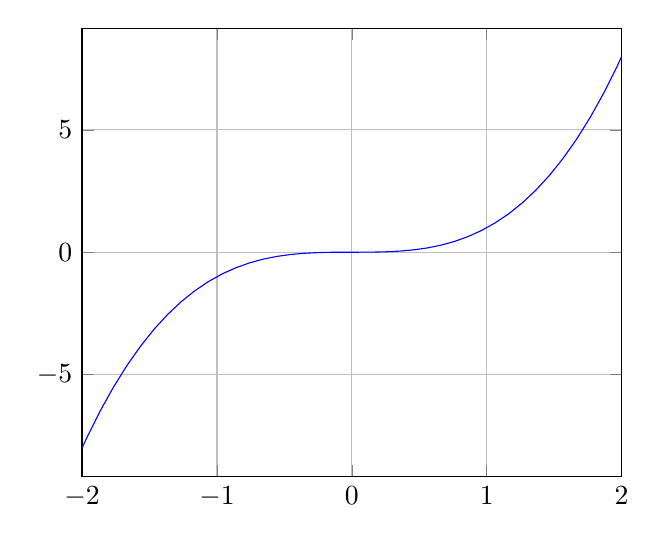
\begin{tikzpicture}
    \begin{axis}[xmin=-2, xmax=2,samples=100, grid]
      \addplot[blue] {x^3};
    \end{axis}
  \end{tikzpicture}
}

\dfn{Even functions}{
  A function is even if $f(-x) = f(x)$.
}
\ex{}{
  $f(x) = x^2$ is even. 
  \\
  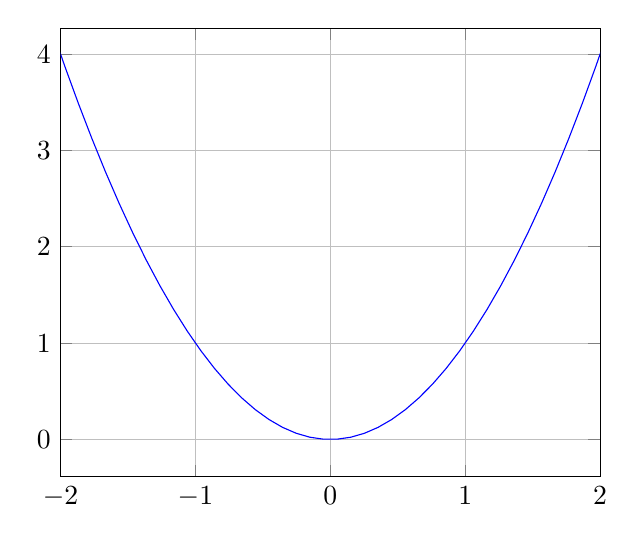
\begin{tikzpicture}
    \begin{axis}[xmin=-2, xmax=2,samples=100, grid]
      \addplot[blue] {x^2};
    \end{axis}
  \end{tikzpicture}
}

\chapter{Topic 2 - Limits and Continuity}

\section{Limits}

\dfn{Limit}{
  The number L is the \textit{limit of the function $f(x)$} as x approaches c if, the values of x get arbitrarily close(but not equal) to c, the values of f(x) approach (or equal) L. We write
  $$ \lim_{x \to c} f(x) = L $$ 
  Moreover, for $ \lim_{x \to c} f(x) = L $ to exist, the left and right hand limits must be equal. Thus, 
  $$ \lim_{x \to c^-} f(x) = \lim_{x \to c^+} f(x) = L $$
} 
\nt{
  If a piecewise function isn't continuous at a point, then the limit at that point does not exist. This is because the right hand and left hand limits aren't equal. 
}

\subsection{Theorems on Limits}

IF k is a constant and the limits of $f(x)$ and $g(x)$ exist as $x \to c$, and $ \lim _{x \to c} f(x) = L $ and $ \lim _{x \to c} g(x) = M $, then:

\thm{The Constant Rule}{
  $$ lim_{x \to c} k = k $$ 
}
\thm{The Constant Multiple Rule}{
  $$ lim_{x \to c} kf(x) = k \lim_{x \to c} f(x) = k \cdot L $$ 
}
\thm{The Sum Rule}{
  $$ lim_{x \to c} (f(x) + g(x)) = \lim_{x \to c} f(x) + \lim_{x \to c} g(x) = L + M $$
}
\thm{The Difference Rule}{
  $$ lim_{x \to c} (f(x) - g(x)) = \lim_{x \to c} f(x) - \lim_{x \to c} g(x) = L - M $$
}
\thm{The Product Rule}{
  $$ lim_{x \to c} (f(x) \cdot g(x)) = \lim_{x \to c} f(x) \cdot \lim_{x \to c} g(x) = L \cdot M $$
}
\thm{The Quotient Rule}{
  $$ lim_{x \to c} \frac{f(x)}{g(x)} = \frac{\lim_{x \to c} f(x)}{\lim_{x \to c} g(x)} = \frac{L}{M} $$
  Provided that $M \neq 0$. Otherwise the limit does not exist.
}
\thm{The Composition Rule}{
  If the limit of $g(x)$ as $x \to c$ is $L$ and $ f(x) $ is continuous at $ x = L$, then
  $$ lim_{x \to c} f(g(x)) = f(\lim_{x \to c} g(x)) = f(L) $$
}
\thm{* THE SQUEEZE THEOREM}{
  If $ f(x) \le g(x) \le h(x) $ and if $ \lim_{x \to c} f(x) = \lim_{x \to c} h(x) = L $, then $ \lim_{x \to c} g(x) = L $.
}

\nt{
  The limit definition of euler's number(e) is:
  $$ e = \lim_{n \to \infty} (1 + \frac{1}{n})^n $$
}

\section{Continuity}

\dfn{Continuity}{
  A function is continuous over an interval if we can draw its graph  without tifting our pencil over that interval. The graph has no holes, breaks, or jumps on a continuous interval. 
  The function y = f(x) is continuous at x = c if: 
  \begin{itemize}
    \item f(c) exists (that is, c is a domain of f(x))
    \item $ \lim_{x \to c} f(x) $ exists
    \item $ \lim_{x \to c} f(x) = f(c) $
  \end{itemize}
  A function is continuous over the closed interval [a,b] if it is continuous at each x such that $ a \le x \le b $ 
  \\
  A function that is not continuous at x = c is said to be discontinuous at x = c. We then call x = c a \textit{point of discontinuity}.
}

\subsection{Theorems on Continuous Functions}
\thm{The Extreme Value Function}{
  If f(x) is continuous over a closed interval [a,b], then f(x) attains a minimum and maximum value somewhere on the interval.
}
\nt{This is important to keep in mind when finding the absolute maximum and minimum of a function. Because there will always be global minima and maxima}

\thm{The Intermediate Value Theorem}{
  If f(x) is continuous over a closed interval [a,b], and if k is any number between f(a) and f(b), then there is at least one number c in [a,b] such that f(c) = k.
}

\thm{The Continuous Functions Theorem}{
  If you have two continuous functions, f(x) and g(x), then:
  \begin{itemize}
    \item $ k \cdot f(x) $ is continuous
    \item $ f(x) + g(x) $ is continuous
    \item $ f(x) - g(x) $ is continuous
    \item $ f(x) \cdot g(x) $ is continuous
    \item $ \frac{f(x)}{g(x)} $ is continuous, provided that $ g(x) \neq 0 $ 
  \end{itemize}
}


\thm{The Composition of Continuous Functions Theorem}{
  If f(x) is continuous at x = c and g(x) is continuous at x = f(c), then $ f(g(x)) $ is continuous at x = c.
}

\chapter{Topic 3 - Differentiation}

\dfn{The definition of the derivitive}{
  At any x in the domain of the function y = f(x), the \textit{derivative} is defined as:
  $$ \lim_{\Delta x \to 0} \frac{f(x + \Delta x) - f(x)}{\Delta x} \text{or} \lim_{\Delta x \to  0} \frac{\Delta y}{\Delta x} $$ 
  A function is said to be \textit{differentiable} at every x for which the limit above exists, and its derivative may be denoted by $ f'(x), y', \frac{dx}{dy}, \text{or} D_xy $. \\ 
  The derivative of $ y = f(x) $ at x = , denoted by $ f'(a) $, is defined as:
  $$ f'(a) = \lim_{h \to 0} \frac{f(a+h) - f(a)}{h} $$ 
}

\section{List of Derivatives}

\begin{equation}
  \frac{d}{dx}k = 0
\end{equation}

\begin{equation}
  \frac{d}{dx} x = 1
\end{equation}

\begin{equation}
  \frac{d}{dx} x^n = nx^{n-1} \text{(The Power Rule)}
  \label{eq:The Power Rule}
\end{equation}

\begin{equation}
  \frac{d}{dx} (u \cdot v) = u \frac{dv}{dx} + v \frac{du}{dx} \text{(The Product Rule)}
  \label{eq:The Product Rule}
\end{equation}

\begin{equation}
  \frac{d}{dx} \frac{u}{v} =  \frac{v \frac{du}{dx} - u \frac{dv}{dx}}{v^2} \text{(The Quotient Rule)}
  \label{eq:The Quotient Rule}
\end{equation}

\begin{equation}
  \frac{d}{dx} e^x = e^x 
  \label{eq:Derivative of e^x}
\end{equation}

\begin{equation}
  \frac{d}{dx} a^x = a^x \ln a
  \label{eq:Derivative of a^x} 
\end{equation}

\begin{equation}
  \frac{d}{dx} \ln x = \frac{1}{x}
  \label{eq:Derivative of ln x} 
\end{equation}

\begin{equation}
  \frac{d}{dx} \log _a x = \frac{1}{x \ln a}
  \label{eq:Derivative of log_a x} 
\end{equation}

\begin{equation}
  \frac{d}{dx} \sin x = \cos x
  \label{eq:Derivative of sin x}
\end{equation}

\begin{equation}
  \frac{d}{dx} \cos x = -\sin x
  \label{eq:Derivative of cos x}
\end{equation}

\begin{equation}
  \frac{d}{dx} \tan x = \sec^2 x
  \label{eq:Derivative of tan x}
\end{equation}

\begin{equation}
  \frac{d}{dx} \cot x = -\csc^2 x
  \label{eq:Derivative of cot x}
\end{equation}

\begin{equation}
  \frac{d}{dx} \sec x = \sec x \tan x
  \label{eq:Derivative of sec x}
\end{equation}

\begin{equation}
  \frac{d}{dx} \csc x = -\csc x \cot x
  \label{eq:Derivative of csc x}
\end{equation}

\begin{equation}
  \frac{d}{dx} \arcsin x = \frac{1}{\sqrt{1-x^2}}
  \label{eq:Derivative of arcsin x}
\end{equation}

\begin{equation}
  \frac{d}{dx} \arccos x = -\frac{1}{\sqrt{1-x^2}}
  \label{eq:Derivative of arccos x}
\end{equation}

\begin{equation}
  \frac{d}{dx} \arctan x = \frac{1}{1+x^2}
  \label{eq:Derivative of arctan x}
\end{equation}

\begin{equation}
  \frac{d}{dx} \cot ^{-1} x = -\frac{1}{1+x^2}
  \label{eq:Derivative of arccot x}
\end{equation}

\begin{equation}
  \frac{d}{dx} \sec ^{-1} x = \frac{1}{x \sqrt{x^2 - 1}}
  \label{eq:Derivative of arcsec x}
\end{equation}

\begin{equation}
  \frac{d}{dx} \csc ^{-1} x = -\frac{1}{x \sqrt{x^2 - 1}}
  \label{eq:Derivative of arccsc x}
\end{equation}

\begin{equation}
  \frac{d}{dx} f^{-1}(x) = \frac{1}{f'(f^{-1}(x))}
  \label{eq:Derivative of f^{-1}(x)}
\end{equation}


\section{The Chain Rule}
\dfn{The Chain Rule}{
  $$ \frac{dy}{dx} = \frac{dy}{du} \cdot \frac{du}{dx} $$
}
\ex{
  $$ \frac{d}{dx} (x^2 + 1)^3 = 3u^2 \cdot \frac{du}{dx} = 3(x^2 + 1)^2 \cdot 2x = 6x(x^2 + 1)^2 $$
}

\section{Differentiablity and Continuity}{
\dfn{The relationship between continuity and differentiability}{
  If $ f $ is differentiable at $ x = a $, then $ f $ is continuous at $ x = a $.
}

\section{Estimating Derivatives}

\qs{Given a table of values, estimate the derivative at a given point.}{
  % 2 by 9 table 
  \begin{center}
    \begin{tabular}{|c|c|c|c|c|c|c|c|c|c|}
      \hline
      $ x $ & 0 & 1 & 2 & 3 & 4 & 5 & 6 & 7 & 8 \\
      \hline
      $ f(x) $ & 98 & 94.95 & 93.06 & 91.90 & 91.17 & 90.73 & 90.45 & 90.28 & 90.17 \\
      \hline
    \end{tabular}
  \end{center}
}

\sol{
  $$ f'(0) \approx \frac{f(1) - f(0)}{1} = \frac{94.95 - 98}{1} = -3.05 $$ 
  $$ f'(1) \approx \frac{f(2) - f(1)}{2 - 1} = \frac{93.06 - 94.95}{1} = -1.89 $$
  $$ f'(2) \approx \frac{f(3) - f(2)}{3 - 2} = \frac{91.90 - 93.06}{1} = -1.16 $$
  $$ f'(3) \approx \frac{f(4) - f(3)}{4 - 3} = \frac{91.17 - 91.90}{1} = -0.73 $$
  $$ f'(4) \approx \frac{f(5) - f(4)}{5 - 4} = \frac{90.73 - 91.17}{1} = -0.44 $$
  And so on...
}

\section{Derivatives of Parametrcally defined functions}

\dfn{Derivatives of Parametrically defined functions}{
  $$ \frac{dy}{dx} = \frac{\frac{dy}{dt}}{\frac{dx}{dt}} $$
  $$ \frac{d^2y}{dx^2} = \frac{d}{dx}(\frac{dy}{dx}) = \frac{\frac{d}{dt}(\frac{dy}{dx})}{\frac{dx}{dt}} $$
}

\section{Implicit Differentiation}

\dfn{Implicit Differentiation}{
  \textit{Implicit Differentiation} is thetechnique we use to find a derivative when y is  not defined explicitly in terms of x but is differentiable.
}
\ex{}{
  If $ x^2 + y^2 - 9 = 0 $, then 
  $$ 2x + 2y \frac{dy}{dx} = 0 $$ 
  And so, 
  $$ \frac{dy}{dx} = -\frac{x}{y} $$
}

\section{The mean value theorem}
\thm{The Mean Value Theorem}{  
  The Mean Value Theorem(MVT) states that If the function f(x) is continuous on the closed interval $ a \le x \le b$ and has a derivative at each point on the open interval $ a < x < b $, then there is at least one number c, $ a < c < b $, such that $ \frac{f(b) - f(a)}{b-a} = f'(c) $.
}
\nt{
  Rolle's Theorem is a special case of the MVT. Where if there is a function f(x) where f(a) = f(b) = k , then there is at least one number c, $ a < c < b $, such that $ f'(c) = 0 $.
}
\qs{}{
  Demonstrate Rolle's Theorem using $ f(x) = x \sin x $ on the interval $ [0, \pi] $.
}
\sol{
  First we check that the conditions of Rolle's Theorem are satisfied. 
  \begin{enumerate}
    \item $ f(x) = x \sin x $ is continuous on the \textit{open interval} $ (0, \pi ) $ and exists for all x in the the closed interval $ [0, \pi] $.
    \item $ f'(x) = \sin x + x \cos x $ exists for all x in the open interval $ (0, \pi) $  
    \item $ f(0) = 0 \sin 0 = 0 $ and $ f(\pi) = \pi \sin \pi = 0 $
  \end{enumerate}
  Since the conditions of Rolle's Theorem are satisfied, there must be at least one number c, $ 0 < c < \pi $, such that $ f'(c) = 0 $ and using a calculator we know that $ c = 2.029 $ (to three decimal places).
}

\section{Indeterminate Forms and L'Hopital's Rule}

\dfn{Indeterminate Forms}{
  An \textit{Indeterminate Form} is an expression that can not be evaluated by substituting the limit. For example, $ \frac{0}{0} $ is an indeterminate form. \\
  The following are all indeterminate forms:
  \begin{itemize}
    \item $ \frac{0}{0} $ 
    \item $ \frac{\infty}{\infty} $ 
    \item $ 0 \cdot \infty $ 
    \item $ \infty - \infty $ 
    \item $ 0^0 $ 
    \item $ 1^\infty $ 
    \item $ \infty^0 $
  \end{itemize}
}

\thm{L'Hospital's Rule}{
  To find the limit of an indeterminate form, we can use L'Hospital's Rule. \\ 
  The rule has several parts:
  \begin{enumerate}
    \item If $ \lim_{x \to a} f(x) = \lim_{x \to a} g(x) = 0  $ and if $ \lim_{x \to a} \frac{f'(x)}{g'(x)} $ exists, then $ \lim_{x \to a} \frac{f(x)}{g(x)} = \lim_{x \to a} \frac{f'(x)}{g'(x)} $  otherwise the rule can't be applied. 
    \item If $ \lim_{x \to a} f(x) = \lim_{x \to a} g(x) = \infty  $ and if $ \lim_{x \to a} \frac{f'(x)}{g'(x)} $ exists, then $ \lim_{x \to a} \frac{f(x)}{g(x)} = \lim_{x \to a} \frac{f'(x)}{g'(x)} $  otherwise the rule can't be applied.
    \item If $ \lim_{x \to \infty} f(x) = \lim_{x \to \infty} g(x) = 0  $ and if $ \lim_{x \to \infty} \frac{f'(x)}{g'(x)} $ exists, then $ \lim_{x \to \infty} \frac{f(x)}{g(x)} = \lim_{x \to \infty} \frac{f'(x)}{g'(x)} $  otherwise the rule can't be applied.
    \item The above rules work for one-sided limits as well. (i.e. $ \lim_{x \to a^-} $, $ \lim_{x \to a^+} $, $ \lim_{x \to + \infty} $, and $ \lim_{x \to - \infty} $ )
    \item You can apply L'Hospital's Rule repeatedly if necessary.
  \end{enumerate}
}

\chapter{Topic 4 - Applications of Differentiation}

\section{Slope and Tangent Lines}
\dfn{Slope}{
  The \textit{slope} of a line at a given point is equal to the derivative of the function at that point.
}
\dfn{Tangent Line}{
  A \textit{tangent line} is a line that touches a curve at a single point and has the same slope as the curve at that point. \\
  The equation of a tangent line is $ y - y_1 = m(x - x_1) $ where $ (x_1, y_1) $ is the point of tangency and m is the slope of the tangent line. 
}

\section{Increasing and Decreasing Functions}

\dfn{The relationship between the derivative the change in a function}{
  Analyzing the signs of the first derivative of a function tells us the intervals over which f(x) is increasing or decreasing. \\
  For intervals where f(x) is increasing, $ f'(x) \ge  0 $ and for intervals where f(x) is decreasing, $ f'(x) \le  0 $.
}
\nt{
  Endpoints of intervals where f(x) is increasing or decreasing are included in the intervals; however, points of discontinuity aren't such.
}

\section{Maximum, Minimum and Inflection Points}

\dfn{Critical Points}{
  A \textit{critical point} of a function f(x) is a point in the domain of f(x) where either $ f'(x) = 0 $ or $ f'(x) $ does not exist.
}

\dfn{Local Maximum}{ 
  A function f(x) has a \textit{local maximum} at $ x = c $ if $ f'(c) = 0 $ and $ f''(x) < 0 $ 
}

\dfn{Local Minimum}{ 
  A function f(x) has a \textit{local minimum} at $ x = c $ if $ f'(c) = 0 $ and $ f''(x) > 0 $ 
}

\dfn{Inflection Point}{
  A function f(x) has an \textit{inflection point} at $ x = c $ if $ f''(c) = 0 $ and $ f''(x) $ switches signs at x = c.  
}
\nt{
  A function is concave up when $ f'' \ge 0 $ and concave down when $ f'' \le 0 $. 
}

\dfn{Global Maximum and Minimum}{
  Using the Extreme Value Theorem, we know that f(x) attains a global maximum and minimum or an interval, thus to solve for the global maximum and minimum we must use the closed interval or candidates test, comparing critical points with endpoints of the interval. 
}

\section{Motion on a line}

\dfn{Position, Velocity, and Acceleration}{
  The \textit{position} of an object at time t is given by the function $ s(t) $. \\
  The \textit{velocity} of an object at time t is given by the function $ v(t) = s'(t) $. \\
  The \textit{acceleration} of an object at time t is given by the function $ a(t) = v'(t) = s''(t) $.
}

\section{Motion along a curve}

\dfn{Position, Velocity, Acceleration Vectors}{
  For parametrically defined functions the following definitions apply: \\
  The \textit{position vector} of an object at time t is given by the function $ \vec{r}(t) = \langle x(t), y(t) \rangle $. \\
  The \textit{velocity vector} of an object at time t is given by the function $ \vec{v}(t) = \vec{r}'(t) = \langle x'(t), y'(t) \rangle $. \\
  The \textit{acceleration vector} of an object at time t is given by the function $ \vec{a}(t) = \vec{v}'(t) = \vec{r}''(t) = \langle x''(t), y''(t) \rangle $.
}

\dfn{Vector Velocity}{\
  The \textit{speed} of an object at time t is given by the function $ \lvert \vec{v}(t) \rvert = \sqrt{x'(t)^2 + y'(t)^2} $.
}

\dfn{Vector Magnitude}{
  The \textit{magnitude} of a vector's velocity $ \vec{v} = \langle x', y' \rangle $ is given by $ \lvert \vec{v} \rvert = \sqrt{x'^2 + y'^2} $.
}

\section{Tangent-Line Approximation}

\dfn{Tangent-Line Approximation}{
  If f'(a) exists, then the \textit{local linear approximation} of f(x) at x = a is \\
  $$ f(x) = f'(a) (x - a) $$ 
  Since the equation of the tangent line to y = f(x) at x = a is \\ 
  $$ y - f(a) = f'(a) (x - a) $$ 
  Therefore, the tangent-line approximation of f(x) at x = a is \\
  $$ f(x) \approx f(a) + f'(a) (x - a) $$ 
}

\section{Related Rates}

If several variables are functions of time or a differing parameter related by an equation, we can  obtain a relation involving their (time) rates of changeby differentiating with respect to t. 

\section{Slope of a Polar Curve}

\dfn{Slope of a Polar Curve}{
  The slope of a polar curve at a point $ P(r, \theta) $ is given by $ \frac{dy}{dx} = \frac{dy/d\theta}{dx/d\theta} = \frac{r \sin \theta + r' \cos \theta}{r \cos \theta - r' \sin \theta} $. This is because the x component of a polar curve is $ x = r\cos \theta $ and the y component is $ y = r \sin \theta $. 
}




\chapter{Topic 5 - Antidifferentiation}

\dfn{Antiderivative}{
  The \textit{antiderivative} or indefinite integral of a function f(x) is a function F(x) such that $ F'(x) = f(x) $. \\
  Since the derivative of a constant is zero, the antiderivative of a function f(x) is a family of functions that differ by a constant. \\
  The antiderivative of f(x) is denoted by $ \int f(x) dx $. \\
  The process of finding the antiderivative of a function is called \textit{antidifferentiation}.\\
  $$ \int f(x) dx = F(x) + C \text{(where C is a constant)} $$
}

\ex{Basic Integrals}{
  \begin{itemize}
    \item $ \int k f(x) dx = k \int f(x) dx $ 
    \item $ \int (f(x) + g(x)) dx = \int f(x) dx + \int g(x) dx $ 
    \item $ \int x^n dx = \frac{x^{n+1}}{n+1} + C $ ( $ n \neq -1 $ )
    \item $ \int \frac{1}{x} dx = \ln \lvert x \rvert + C $ 
    \item $ \int e^x dx = e^x + C $ 
    \item $ \int a^x dx = \frac{a^x}{\ln a} + C $ 
    \item $ \int \sin x dx = -\cos x + C $
    \item $ \int \cos x dx = \sin x + C $ 
    \item $ \int \tan x dx = -\ln \lvert \cos x \rvert + C $ 
    \item $ \int \sec^2 x dx = \tan x + C $
    \item $ \int \csc^2 x dx = -\cot x + C $  
    \item $ \int \sec x \tan x dx = \sec x + C $ 
    \item $ \int \csc x \cot x dx = -\csc x + C $ 
    \item $ \int \frac{1}{x^2 + a^2} dx = \frac{1}{a} \tan^{-1} \frac{x}{a} + C $ 
    \item $ \int \frac{1}{\sqrt{a^2 - x^2}} dx = \sin^{-1} \frac{x}{a} + C $ 
    \item $ \int \frac{1}{\sqrt{x^2 - a^2}} dx = \cos^{-1} \frac{x}{a} + C $
    \item $ \int f^{-1} (x) = x f^{-1} (x) - F(f^{-1}(x)) + C dx $
  \end{itemize}
}


\section{Methods of Integration}

\thm{Integration by Substitution}{
  If $ u = g(x) $ is a differentiable function whose range is an interval I and f is continuous on I, then \\
  $$ \int f(g(x)) g'(x) dx = \int f(u) du $$
}

\thm{Integration by Partial Fractions}{
  The method of partial fractions makes it possible to express a rational function $ \frac{f(x)}{g(x)} $ as a sum of simpler fractions. \\
  If the degree of f(x) is less than the degree of g(x), then the rational function $ \frac{f(x)}{g(x)} $ can be expressed as a sum of partial fractions. \\
  ex: $ \frac{2x^2 + 5x + 1}{x^3 + 2x^2} = \frac{A}{x} + \frac{B}{x^2} + \frac{C}{x+2} $ \\
  To find the constants A, B, and C, we can multiply both sides by the denominator and then substitute values for x that make the other terms zero. \\
  ex: $ 2x^2 + 5x + 1 = A(x^2)(x+2) + B(x+2) + C(x^2) $ \\
  $ x = 0 \Rightarrow 1 = 2C \Rightarrow C = \frac{1}{2} $ \\
  $ x = -2 \Rightarrow 4 = 4A \Rightarrow A = 1 $ \\
  $ x = -1 \Rightarrow -2 = -2B \Rightarrow B = 1 $ \\
  Therefore, $ \frac{2x^2 + 5x + 1}{x^3 + 2x^2} = \frac{1}{x} + \frac{1}{x^2} + \frac{1}{2(x+2)} $ \\
  Thus,
  $$ \int \frac{2x^2 + 5x + 1}{x^3 + 2x^2} dx = \int \frac{1}{x} dx + \int \frac{1}{x^2} dx + \int \frac{1}{2(x+2)} dx $$
}

\thm{Integration by Parts}{
  If u and v are differentiable functions, then \\
  $$ \int u dv = uv - \int v du $$ 
  The acronym LIPET is used to remember the order of integration by parts, choose u in the followin g order. \\
  L - Logarithmic \\
  I - Inverse Trigonometric \\
  P - Polynomial \\
  E - Exponential \\
  T - Trigonometric
}
\qs{Find $ \int  x \cos x dx$ }{Using integrations by parts}

\sol{
  We let u = x and dv = $ \cos x dx $. Then du = dx and v = sinx \\
  $$ \int x \cos x dx = x \sin x - \int \sin x dx = x \sin x + \cos x + C $$
}

\thm{The Tic-Tac-Toe Method}{
  This method of integration is extremely useful when repeated integration of parts is necessary. To integrate $ \int u(x) v(x) dx $, we construct a table where u' is the derivative of u(x) and $v_1(x)$ is the antiderivative of v(x) as follows: 
  % 3 column table
  \begin{center}
    \begin{tabular}{|c|c|c|}
      \hline
      u(x) & + & $ v(x) $ \\
      \hline
      $ u' $ & - & $ v_1(x) $ \\
      \hline
      $ u'' $ & + & $ v_2(x) $ \\
      \hline
      $ u''' $ & - & $ v_3(x) $ \\
      \hline
      $ u^{(4)} $ &  &  \\
      \hline
    \end{tabular}
  \end{center}

  Such that: 
  $$ \int u(x) v(x) dx = u(x)v_1(x) - u'(x)v_2(x) + u''(x)v_3(x) - u'''(x)v_4(x) + \cdots $$
  * this method is also called the tabular method!
}



\chapter{Topic 6 - Definite Integrals}

\dfn{The Fundamental Theorem of Calculus}{
If f is continuous on the closed interval [a,b] and F' = f, then according to the FTC,
$$ \int_a^b f(x) dx = F(b) - F(a) $$
}

\section{Reimann Sums}

\dfn{Reimann Sum}{
  Let $ f $ be defined on the interval $ [a,b] $ and let $ P = \{ x_0, x_1, \cdots, x_n \} $ be a partition of $ [a,b] $, where $ a = x_0 < x_1 < \cdots < x_n = b $. Let $ \Delta x_i = x_i - x_{i-1} $ be the length of the ith subinterval. Let $ c_i $ be any point in the ith subinterval $ [x_{i-1}, x_i] $. Then the sum
  $$ \sum_{i=1}^n f(c_i) \Delta x_i $$
  is called a Reimann Sum for f on [a,b] associated with the partition P and the choice of $ c_i $ in the ith subinterval. 
}

\thm{Approximations of the definite integral using Reimann Sums}{
  Left Sum: $ f(x_0) \Delta x_1 + \ldots $ \\
  Right Sum: $ f(x_1) \Delta x_1 + \ldots $ \\
  Midpoint Sum: $ f(\frac{x_0 + x_1}{2}) \Delta x_1 + \ldots $ \\
  Trapezoidal Sum: $ \frac{1}{2} (f(x_0) + f(x_1)) \Delta x_1 + \ldots $ \\
}



\chapter{Topic 7 - Applications of Integration to Geometry}

\section{Finding Area using integrals}

\thm{Finding Area with integrals}{
  $$ A = \int _a^b f(x)dx $$ 
  The area between two curves is: 
  $$ \int _a^b [g(x) - f(x)]dx \text{(if there are no points of intersection, otherwise)} $$ 
  $$ \int _a^b [g(x) - f(x)]dx - \int _b^c [f(x) - g(x)] dx $$ 
}

\thm{The Region bounded by a Polar Curve}{
  $$ A = \frac{1}{2} \int r^2 d \theta $$ 
}

\section{Finding Volume using integrals}

\thm{Finding Volume of Solids with known cross sections}{
  $$ V = \int A(x) dx $$
}

\thm{Finding the Volume of Disks, Washers, and Shells}{
  Disk: $ \Delta V = \pi r^2 \Delta x $ and $ V = \pi \int _a^b r^2 dx $. \\
  Washer: $ \Delta V = \pi  R^2 \Delta x - \pi r^2 \Delta x$ and $ V = \pi \int _a^b (R^2 - r^2) dx $. \\
  Shells: $ \Delta V = 2 \pi rh \Delta x $ and $ V = 2 \pi \int _a^b rhdx $ 
}

\section{Arc Length}

\thm{The Formula for Arc Length}{
  $$ s = \int _a^b \sqrt{1 + \frac{dy}{dx}^2} dx $$
  For parametric functions:
  $$ s = \int _a^b \sqrt{\frac{dx}{dt}^2 + \frac{dy}{dt}^2} dt $$ 
}

\section{Improper Integrals}

\dfn{Improper Integrals}{
  There are two kinds of improper integrals: 
  \begin{itemize}
    \item Those in which at least one fo the limits of integration is infinite (the interval is not bounded)
    \item Those of the type $ \int _a^b f(x) dx $, where f(x) has a point of discontinuity (becoming infinite) at x = c, $ a \le c \le b $ ( the function is not bounded). 
  \end{itemize}
}

\thm{The comparison test for improper integral}{
  If $ f(x) \le g(x) $ and both $ \int _a^b f(x) dx $ and $ \int _a^b g(x) dx $ are improper integrals with g(x) converging, then $ \int _a^b f(x) dx $ converges. \\
  If $ f(x) \ge g(x) $ and both $ \int _a^b f(x) dx $ and $ \int _a^b g(x) dx $ are improper integrals with g(x) diverging, then $ \int _a^b f(x) dx $ diverges. \\
}


\chapter{Topic 8 - More Applications of Integration} 

\section{Average Value of a Function}

\dfn{Average Value of a Function}{
  $$ f_{avg} = \frac{1}{b-a} \int _a^b f(x) dx $$
}

\section{Distance a particle moves on a curve}

\thm{Distance a particle moves on a parametric curve}{
  $$ s = \int _a^b \sqrt{\frac{dx}{dt}^2 + \frac{dy}{dt}^2} dt $$
}


\chapter{Topic 9 - Differential Equations} 

\dfn{Differential Equation}{
  An equation that involves a derivative is called a differential equation. 
}

\section{Rate of Change + Slope Fields}

\dfn{Rate of Change}{
  The rate of change of a quantity y with respect to another quantity x is defined as the derivative of y with respect to x.
}

\dfn{Slope Field}{
  A slope field is a graph of the slopes of a differential equation. This is a basically a graph of every derivative at many points on a graph. 
}


\section{Derivatives of Implicitly defined functions}

\thm{Derivatives of Implicitly defined functions}{
  ex: $ x^2 + y^2 = 25 $ \\
  $$ 2x + 2y \frac{dy}{dx} = 0 $$ 
  $$ \frac{dy}{dx} = - \frac{x}{y} $$
  Now for implementing implicit functions in slope fields we can just plug in the x and y values into the derivative.
}

\section{Euler's Method}

\thm{Euler's Method}{
  $$ y_{n+1} = y_n + f(x_n, y_n) \Delta x $$
  Where $ \Delta x = \frac{b-a}{n} $ and $ x_n = a + n \Delta x $ 
}

\end{document}
